\documentclass{beamer}
\usepackage{relsize}
\usepackage{color}

\usepackage{listings}
\usetheme{CambridgeUS}
%\usepackage{beamerthemesplit} % new
\usepackage{enumitem}
\usepackage{amsmath}                    % See geometry.pdf to learn the layout options.
\usepackage{amsthm}                   % See geometry.pdf to learn the layout options. There
\usepackage{amssymb}                    % See geometry.pdf to learn the layout options.
\usepackage[utf8]{inputenc}
\usepackage{graphicx}
\usepackage[english,bulgarian]{babel}

\usepackage{caption}
\usepackage{tikz}
\usetikzlibrary{shapes,arrows,positioning,calc,positioning,fit,chains}

\usetheme{CambridgeUS}
\usecolortheme{crane}

\lstset{language=Haskell,
                basicstyle=\ttfamily\small,
                keywordstyle=\color{blue}\ttfamily,
                stringstyle=\color{red}\ttfamily,
                commentstyle=\color{green}\ttfamily,
                morecomment=[l][\color{magenta}]{\#}
}

\newtheorem{mydef}{Дефиниция}[section]
\newtheorem{lem}{Лема}[section]
\newtheorem{thm}{Твърдение}[section]

\DeclareMathOperator{\restrict}{\upharpoonright}

\setitemize{label=\usebeamerfont*{itemize item}%
  \usebeamercolor[fg]{itemize item}
  \usebeamertemplate{itemize item}}

\setbeamercovered{transparent}

\captionsetup{font=tiny} 


\tikzset{
block/.style = {draw, fill=white, rectangle,align = center},
entry/.style = {draw, fill=black, circle, radius=3em},
condition/.style = {draw, fill=white, diamond, align = center,node distance=3cm},
fork/.style = {draw, fill=black, circle,inner sep=1pt},
lnode/.style={rectangle split, rectangle split parts=3,draw, rectangle split horizontal},
treenode/.style = {align=center, inner sep=0pt, text centered, circle, font=\sffamily\bfseries, draw=black, fill=white, text width=1.5em}
}


\begin{document}
\title[Рекурсия]{Рекурсия с връщане назад}
\frame{\titlepage}

\section{Рекурсия}
\subsection{}

\begin{frame}
  \centerline{Да си припомним рекурсията}
\end{frame}


\begin{frame}[fragile]
  \frametitle{Разлагане на прости делители}


  \begin{columns}[t]
    \begin{column}{0.7\textwidth}
  
      \begin{lstlisting}
firstdivisor x = divisorhelp x 2

divisorhelp x k 
      | k >= x = x
      | mod x k == 0 = k
      | otherwise = divisorhelp x (k+1)                    
      \end{lstlisting}

  
    \end{column}
    \begin{column}{0.3\textwidth}
      \relscale{0.6}
      \begin{flushright}

        $351509=17.$$\stackrel{20677}{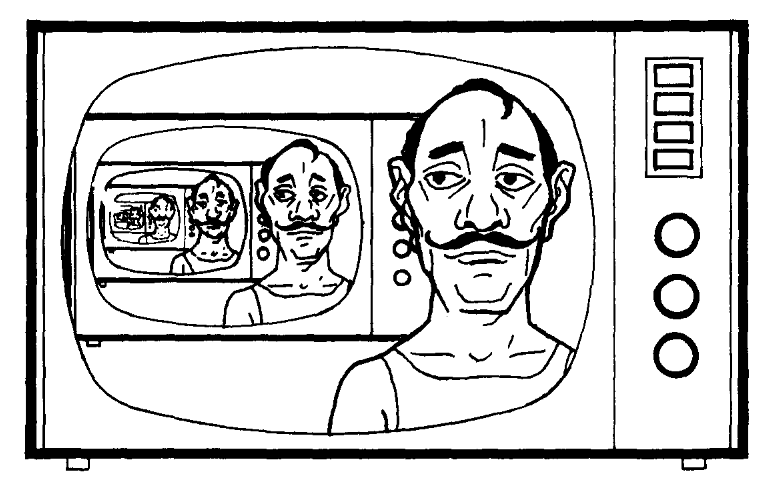
\includegraphics[width=2cm]{images/rec_wirt}}$
        
        $20677=23.$$\stackrel{899}{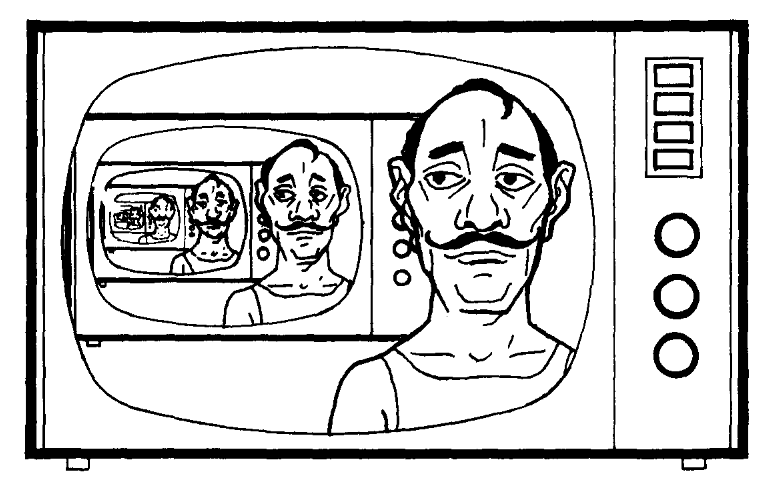
\includegraphics[width=1.6cm]{images/rec_wirt}}$
        
        $899=29.$$\stackrel{31}{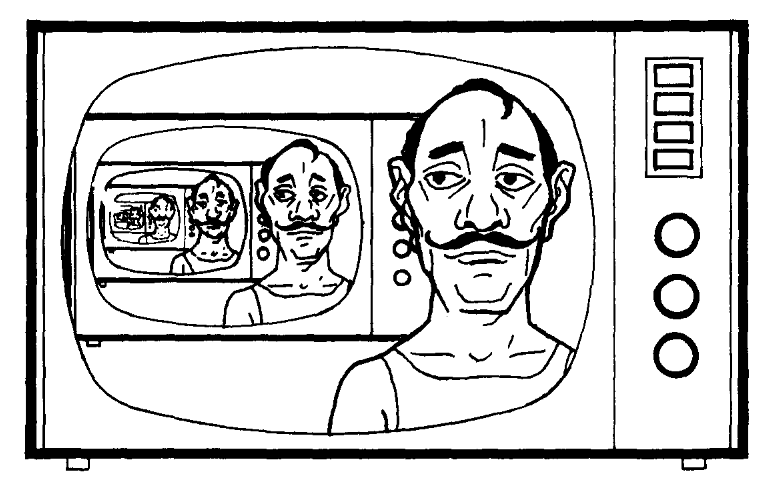
\includegraphics[width=1.2cm]{images/rec_wirt}}$
        
        ...    
      \end{flushright}
      \relscale{1}
      
    \end{column}
  \end{columns}
  
\end{frame}


\begin{frame}[fragile]
  \frametitle{Разлагане на прости делители}

  $351509=17.$$\stackrel{20677}{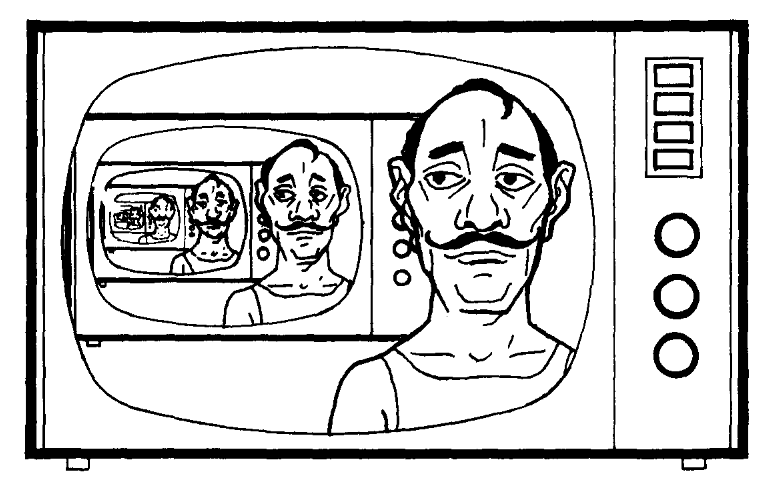
\includegraphics[width=2cm]{images/rec_wirt}}$

\bigskip

\begin{lstlisting}
divisors 1 = []
divisors x = fistdivisor x : 
             divisors (div x (fistdivisor x))      
\end{lstlisting}

  
\end{frame}


\begin{frame}[fragile]
  \frametitle{Бързо сортиране}

  \begin{center}
    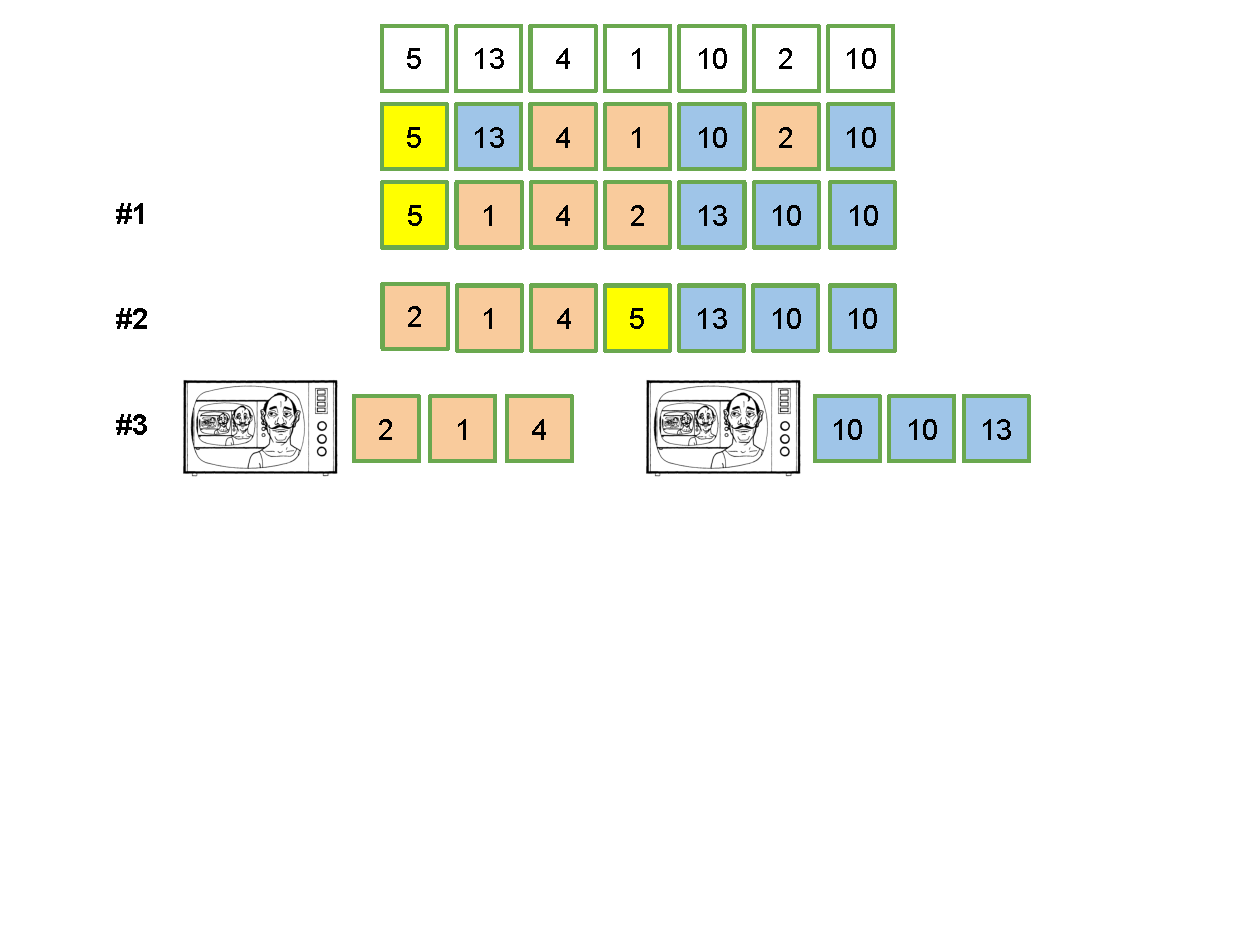
\includegraphics[width=12cm]{images/qsort}
 \end{center}
   
\end{frame}

\vspace*{-0.5cm}


\begin{frame}[fragile]
  \frametitle{Бързо сортиране}

  \begin{center}
    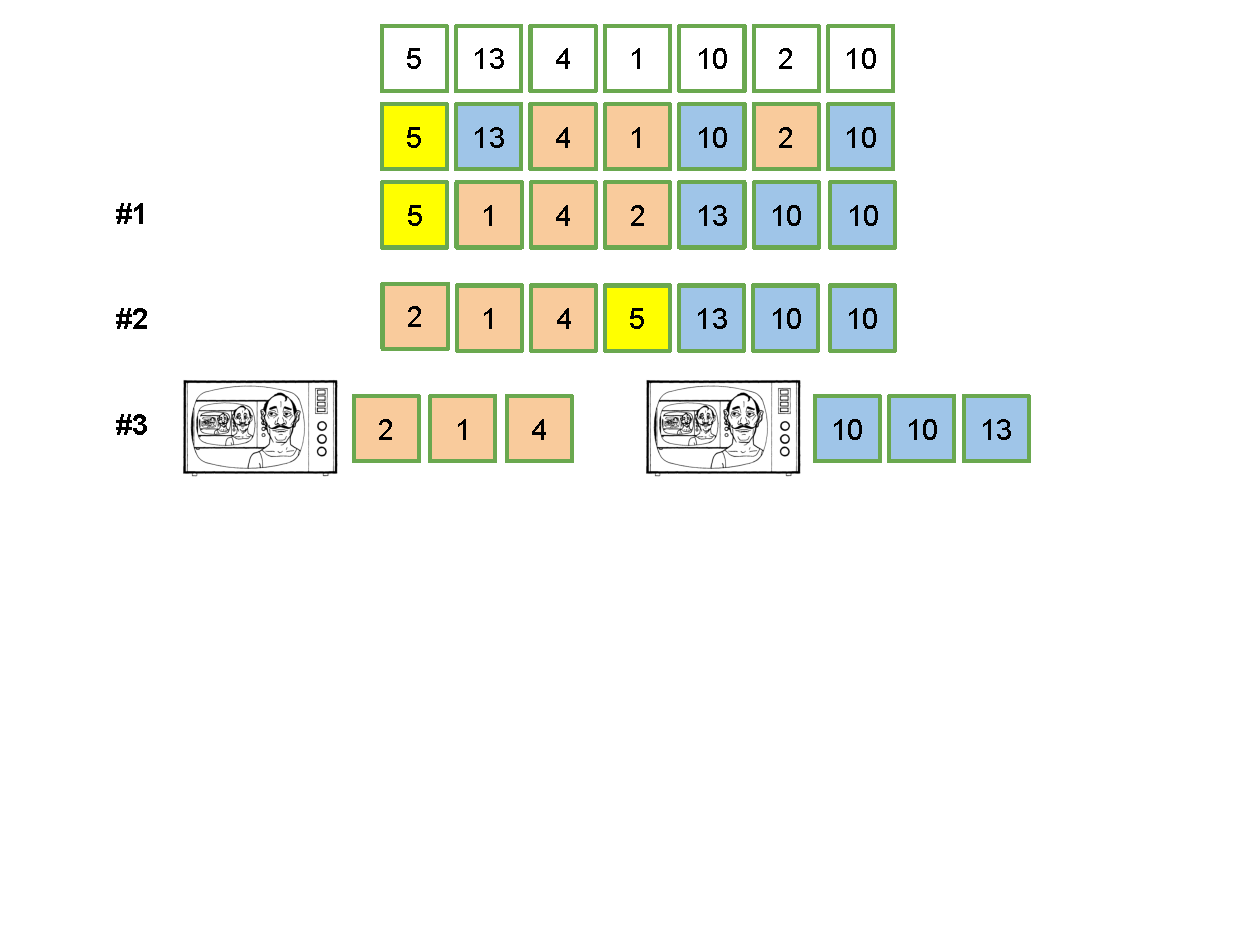
\includegraphics[width=6cm]{images/qsort}
 \end{center}
   
\vspace*{-2cm}

\begin{lstlisting}
  split [] _ = ([], [])
  split (x:xs) pivot 
      | x < pivot = (x:smaller, larger)
      | otherwise = (smaller, x:larger)
      where (smaller, larger) = split xs pivot
  
  qsort [] = []
  qsort (x:xs) = qsort smaller ++ [x] ++ qsort larger
      where (smaller, larger) = split xs x
  \end{lstlisting}
  

\end{frame}


\begin{frame}
  \centerline{Търсене на път в лабиринт}
\end{frame}



\begin{frame}[fragile]
  \frametitle{Задачата}
  %\vspace*{-25pt}
  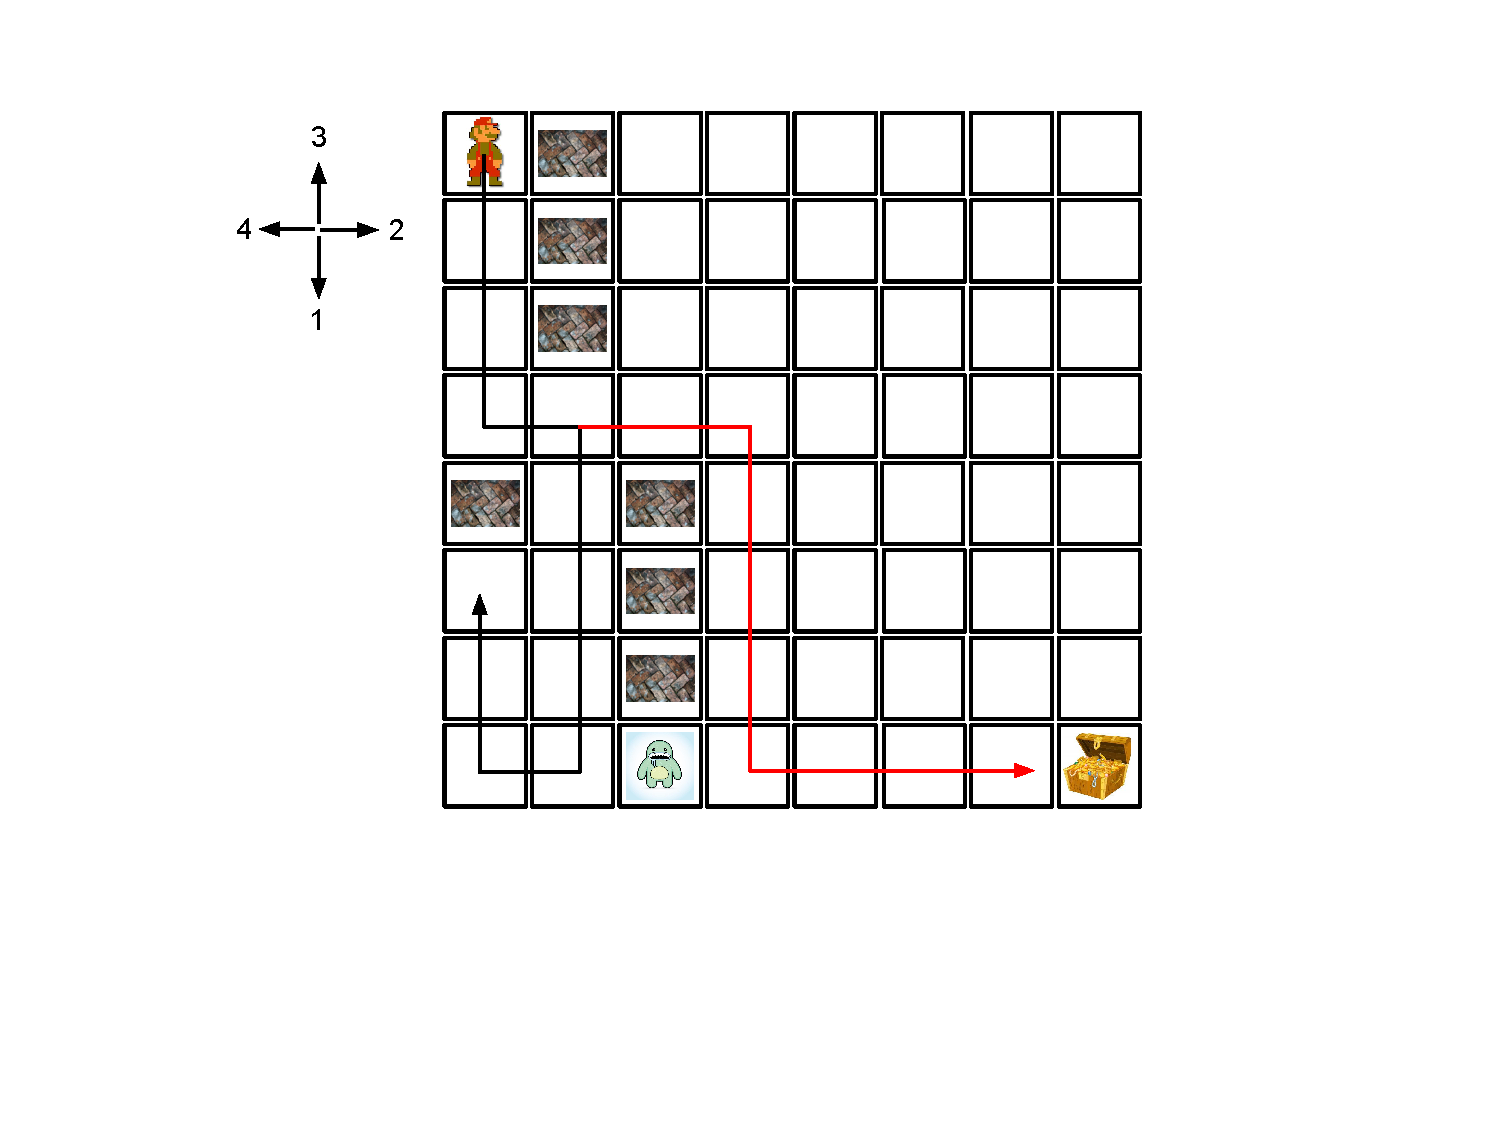
\includegraphics[width=12cm]{images/lab_sol}
\end{frame}

\begin{frame}[fragile]
  \frametitle{Търсене}
  %\vspace*{-25pt}
  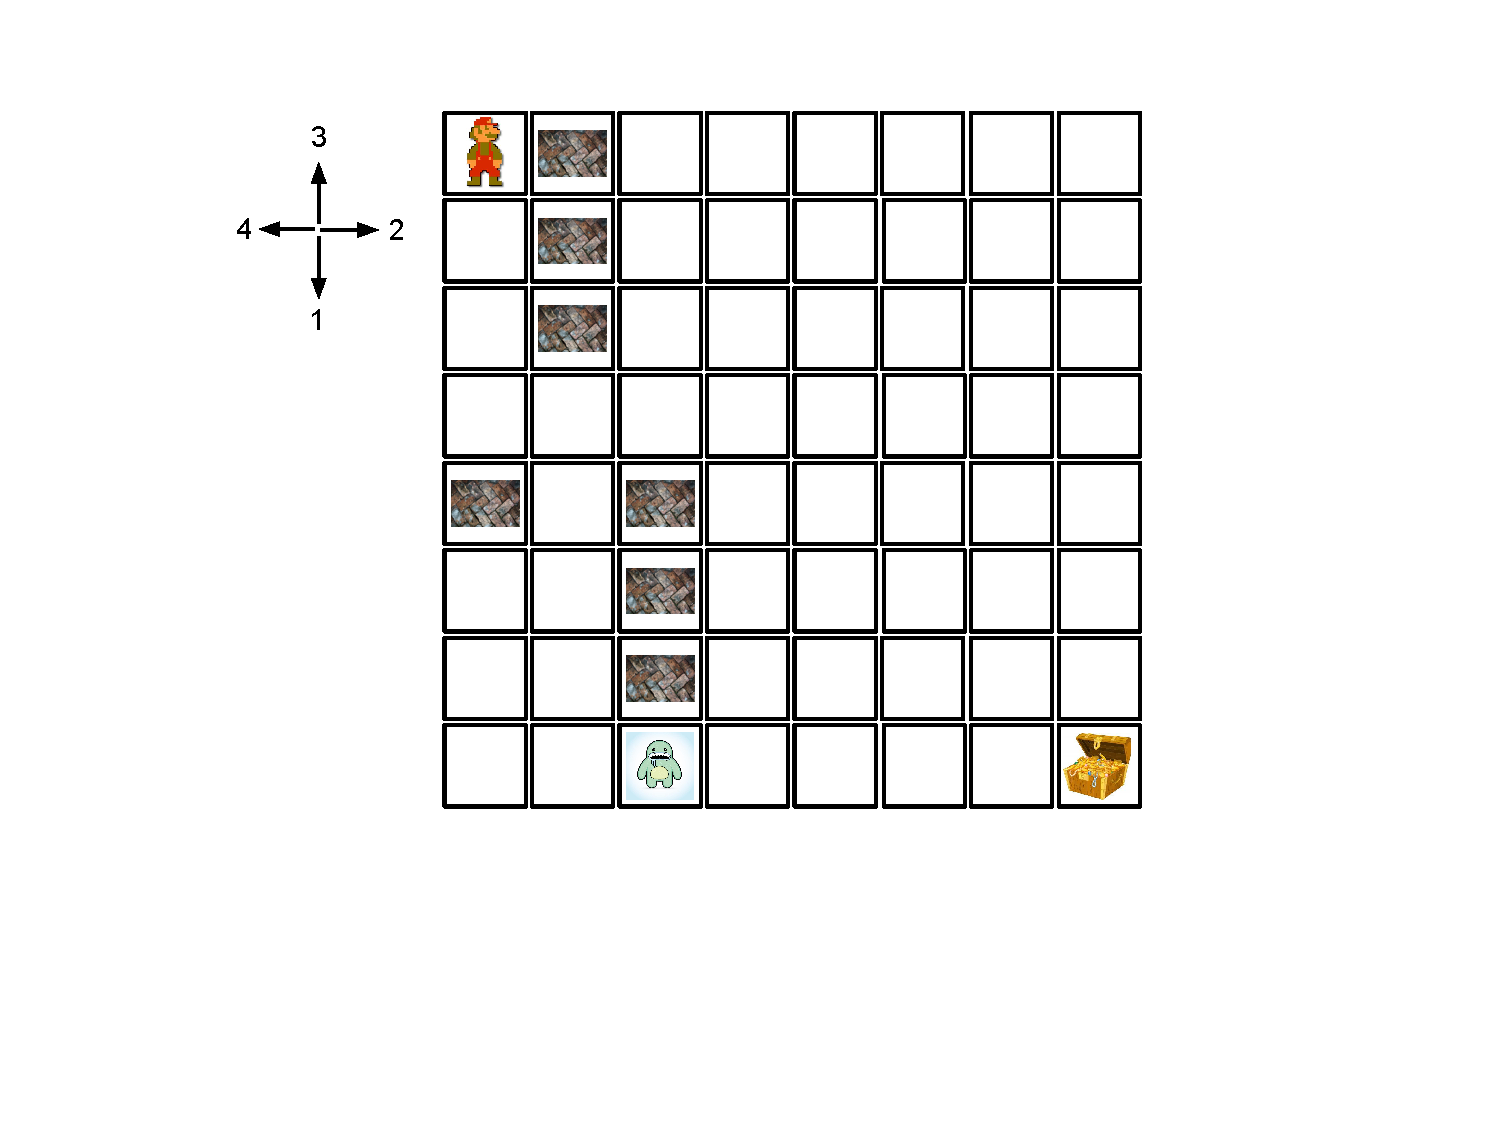
\includegraphics[width=12cm]{images/lab_00}
\end{frame}

\begin{frame}[fragile]
\frametitle{Търсене}
%\vspace*{-25pt}
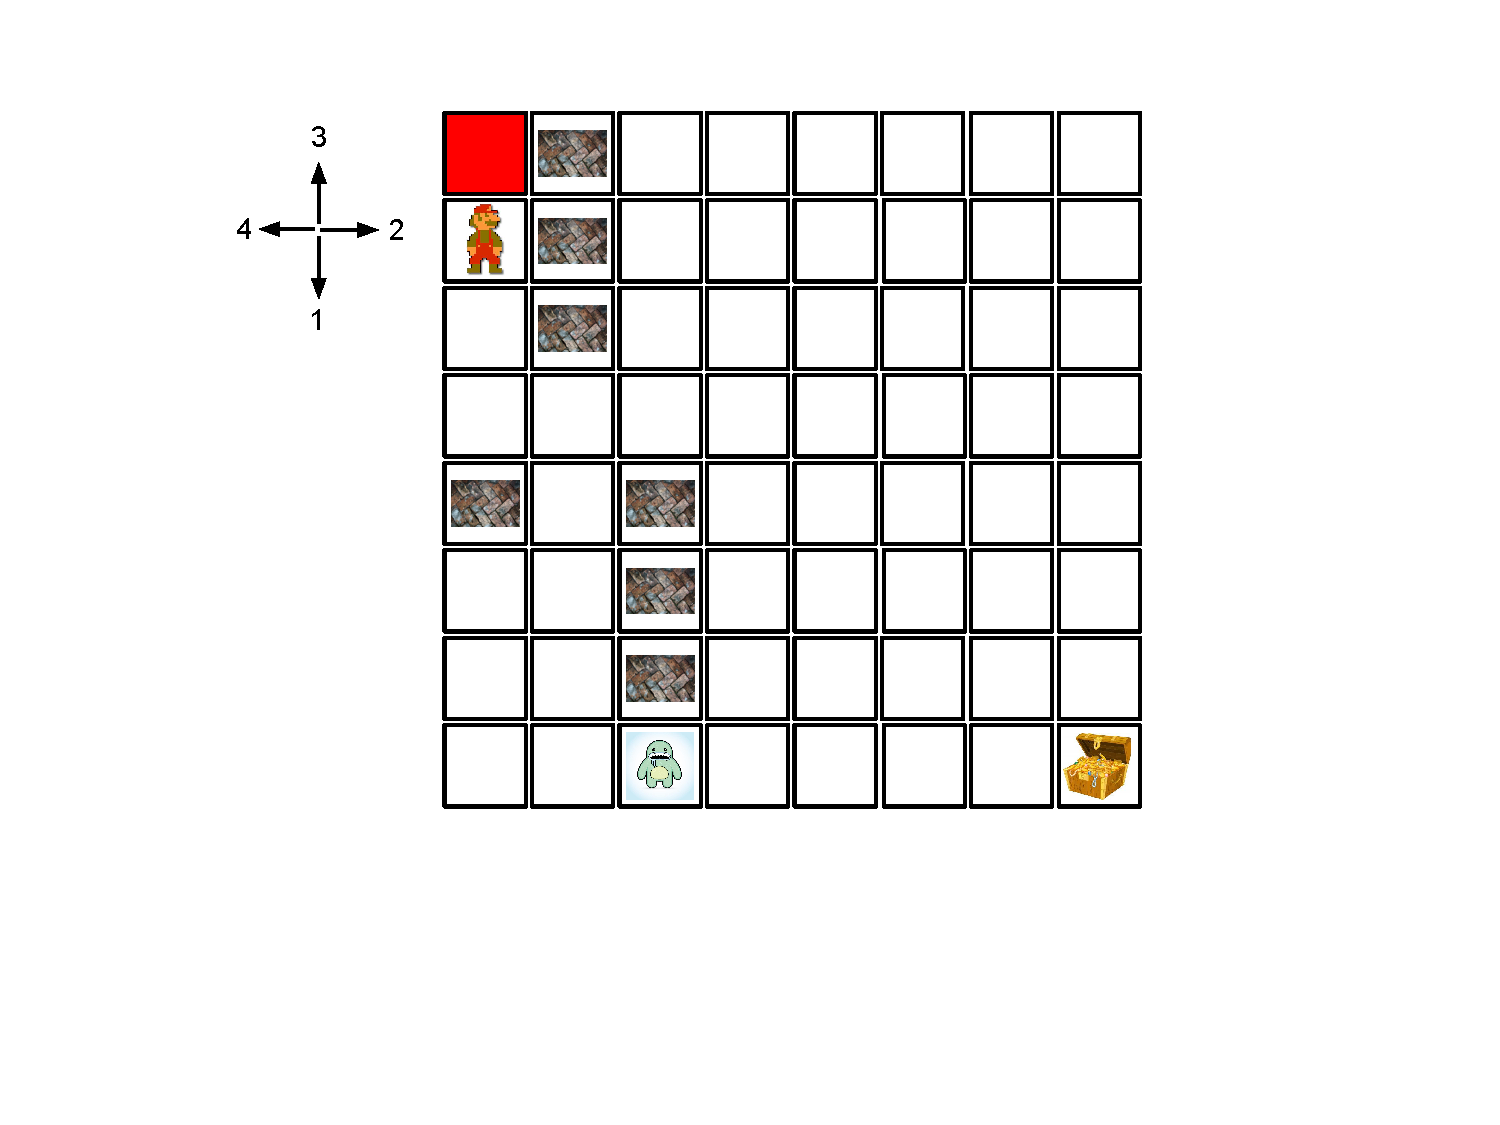
\includegraphics[width=12cm]{images/lab_01}
\end{frame}

\begin{frame}[fragile]
\frametitle{Търсене}
%\vspace*{-25pt}
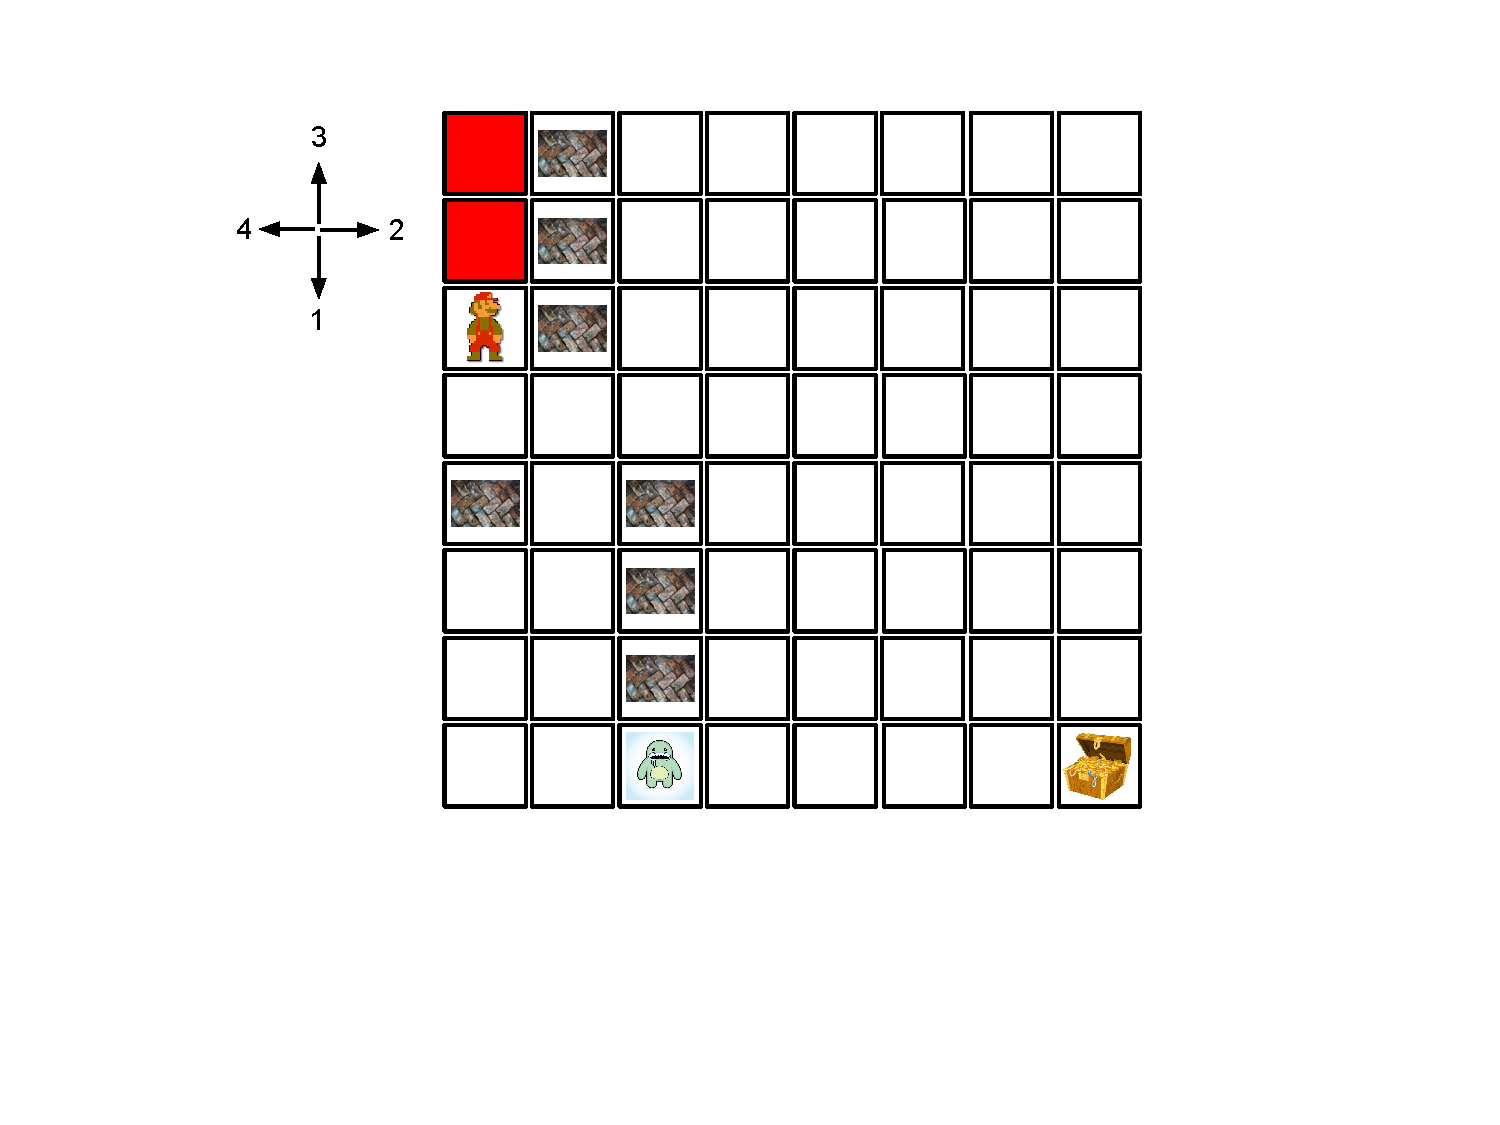
\includegraphics[width=12cm]{images/lab_02}
\end{frame}


\begin{frame}[fragile]
\frametitle{Търсене}
%\vspace*{-25pt}
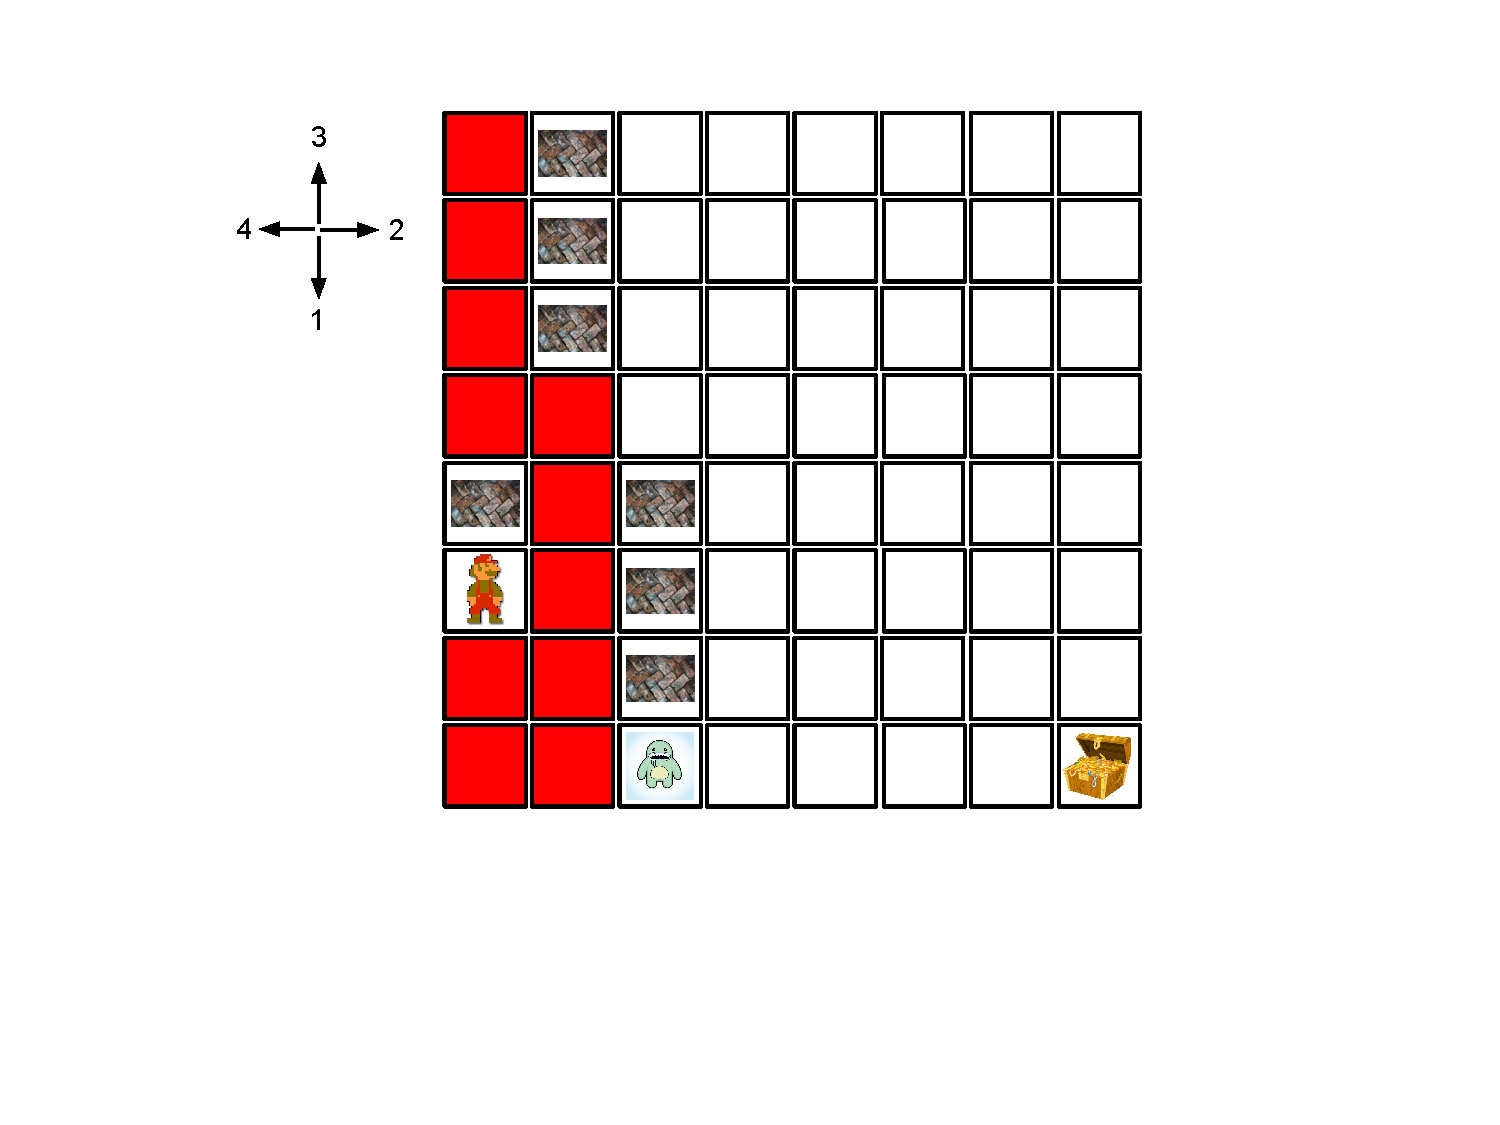
\includegraphics[width=12cm]{images/lab_dead1}
\end{frame}



\begin{frame}[fragile]
\frametitle{Търсене}
%\vspace*{-25pt}
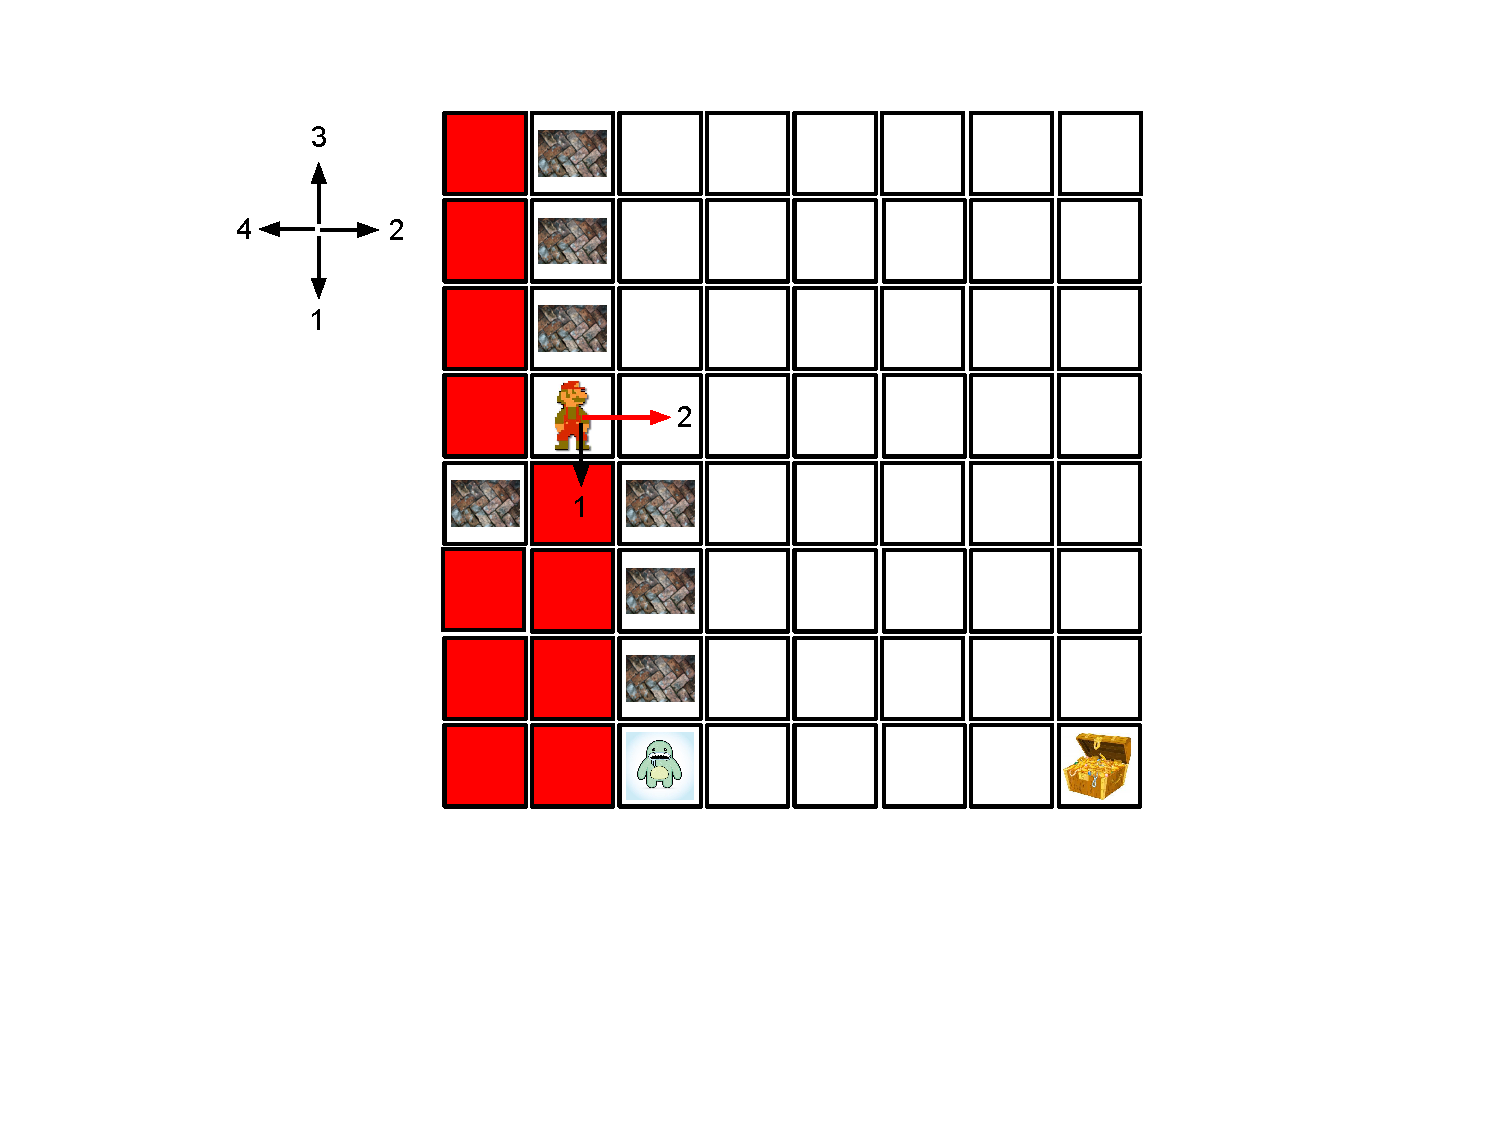
\includegraphics[width=12cm]{images/lab_choice_01}
\end{frame}
  


\begin{frame}[fragile]
  \frametitle{Пълно изчерпване}


\begin{tikzpicture}[remember picture,overlay]
  \node[xshift=80mm,yshift=-12mm,anchor=north west] at (current page.north west){%
  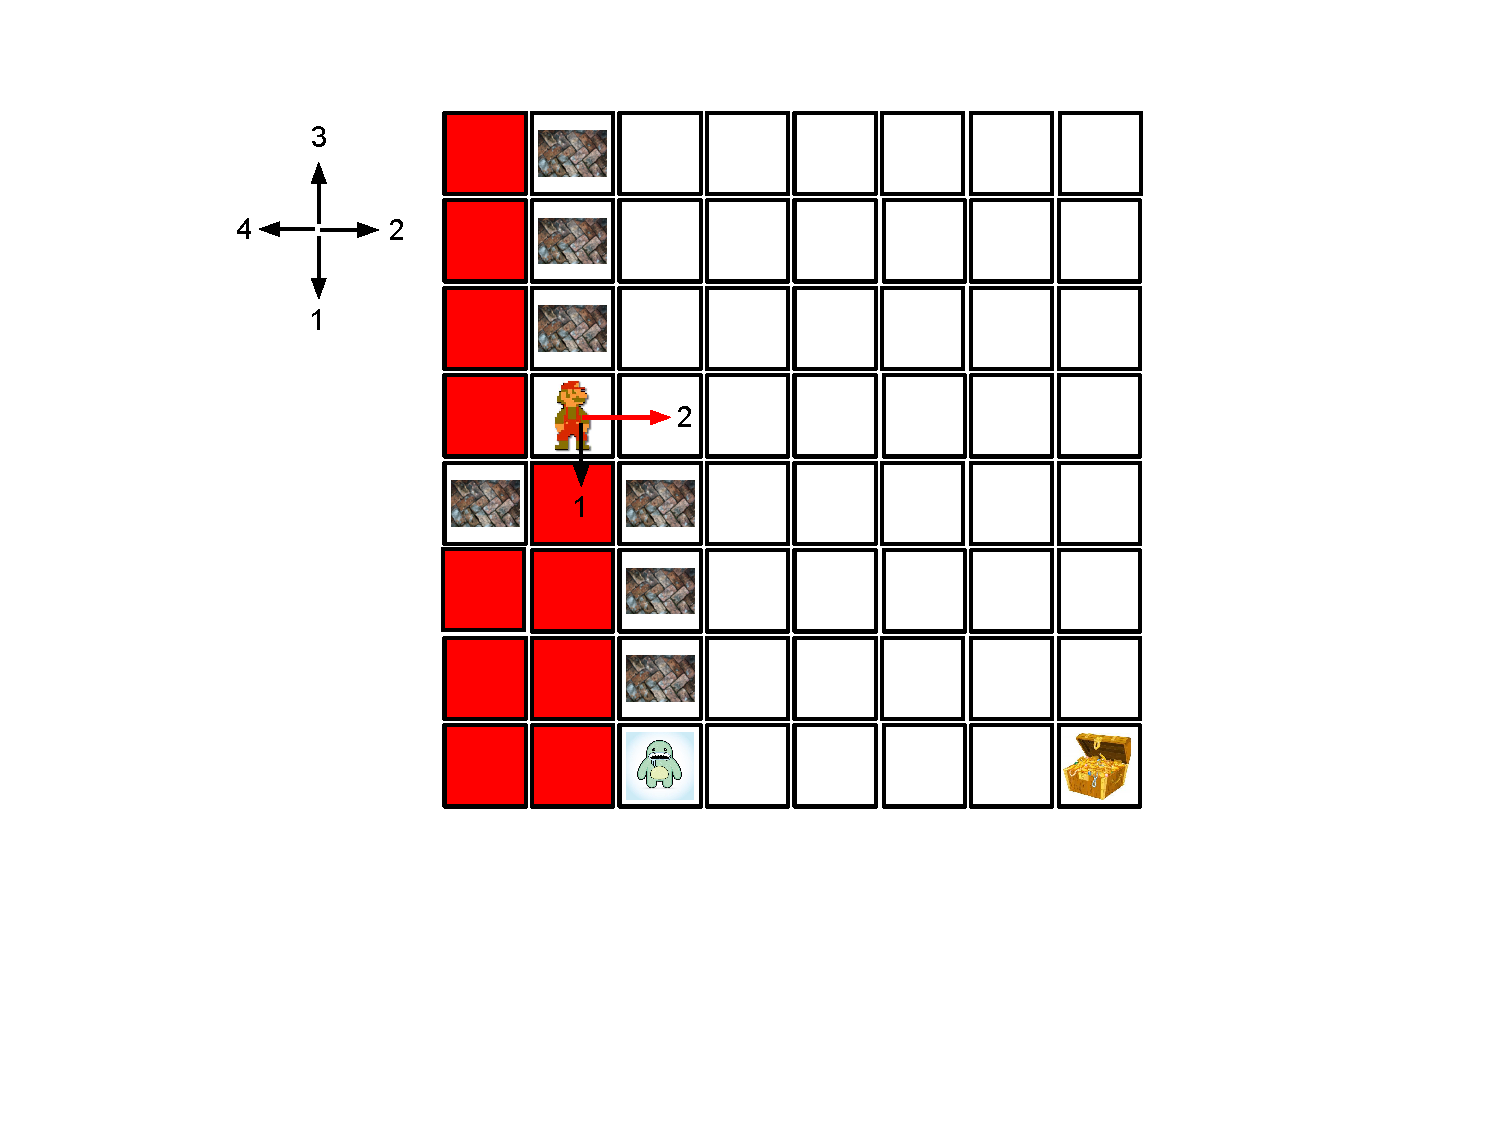
\includegraphics[width=55mm]{images/lab_choice_01}};
\end{tikzpicture}
     
\begin{itemize}
  \item Не е елегантно, засега върши работа
\end{itemize}

\begin{lstlisting}
  --findGold :: game visited -> path
  findGold :: Maybe Game -> [Pos] -> [Pos]
  findGold Nothing _ = []
  findGold (Just g@(Game p w)) visited
      | foundGold g = [p]
      | (stuck g) || (elem p visited) = []
      | downpath /= [] = p : downpath
      | rightpath /= [] = p : rightpath
      | uppath /= [] = p : uppath
      | leftpath /= [] = p : leftpath
      where downpath = findGold (down g) (p:visited)
            rightpath = findGold (right g) (p:visited)
            uppath = findGold (up g) (p:visited)
            leftpath = findGold (left g) (p:visited)  
\end{lstlisting}
  

\end{frame}

\subsection{Опашкова рекурсия}

\begin{frame}
  \centerline{Опашкова рекурсия}
\end{frame}

\begin{frame}[fragile]
  \frametitle{Обобщение на ``цикъл''}

\begin{figure}
  \scalebox{0.5}{
    \begin{tikzpicture}[auto, node distance=1.5cm,>=latex']
    \node [entry, name=start](start){};
    \node [block,name=init, below of = start] (init)
       {Инициализация на\\ $v_0,..,v_n$};
    \node [fork,name=test1fork,below of = init,node distance = 2cm]{};
    \node [condition,name=test1, below of = test1fork,node distance = 3cm] (test1) {Условие \\ $C(v_0,..,v_n)$};
    \node [block,name=inc,right of = test1, node distance = 6.5cm] (inc) {Операции \\$(v_0^i,..,v_n^i) \rightarrow (v_0^{i+1},..,v_n^{i+1})$};
    \node [fork,name=endfork,below of = test1, node distance = 3cm]{};
    \node [entry, name=end, below of = endfork, node distance = 1cm](end){};

    \node [name=cut1, left of = test1fork, node distance = 2cm](cut1){1};
    \node [name=cut2, left of = endfork, node distance = 2cm](cut2){2};

    \draw [->] (start) -- (init);
    \draw [-] (init) -- (test1fork);
    \draw [->] (test1fork) -- (test1);
    \draw [->] (test1) -- node{true} (inc);
    \draw [->] (inc) |- (test1fork);
    \draw [-] (test1) -- node []{false}(endfork);
    \draw [->] (endfork) -- (end);

    \draw [-,dashed] (cut1) -- (test1fork);
    \draw [-,dashed] (cut2) -- (endfork);
    \end{tikzpicture}
  }
\end{figure}

$(v_0^0,..,v_n^0) \rightarrow (v_0^1,..,v_n^1) \rightarrow  ... \rightarrow  (v_0^k,..,v_n^k)$

\end{frame}


\begin{frame}[fragile]
  \frametitle{Опашкова рекурсия}

\begin{lstlisting}
suml :: Num a => [a] -> a
suml [] = 0
suml (x:xs) = x + suml xs

sumiter :: Num a => [a] -> a -> a
sumiter [] current = current
sumiter (x:xs) current = sumiter xs (current + x)

>sumiter [1,2,3,4] 0
\end{lstlisting}


\end{frame}


\begin{frame}[fragile]
  \frametitle{Опашкова рекурсия}

\begin{lstlisting}[basicstyle=\ttfamily\tiny]
splithelp :: Ord a => [a] -> a -> ([a], [a]) -> ([a], [a])

splithelp [] _ current = current
splithelp (x:xs) pivot (smaller, larger) 
                              = splithelp xs pivot (smaller', larger')
    where (smaller', larger') = if x < pivot 
                                then (x:smaller, larger) 
                                else (smaller, x:larger)
\end{lstlisting}


\end{frame}


\begin{frame}[fragile]
    \frametitle{}
  
  \centerline{Благодаря за вниманието!}
\newcommand{\license}[1]{
  \begin{tikzpicture}[remember picture,overlay]
      \node[xshift=0mm,yshift=13mm,anchor=south east] at (current page.south east)
      {\tiny{Материалите са разработени от Калин Георгиев за курсовете по програмиране на ФМИ, СУ}};
      \node[xshift=0mm,yshift=10mm,anchor=south east] at (current page.south east)
      {\tiny{Creative Commons Attribution-NonCommercial-ShareAlike 4.0 International}};
      \node[xshift=0mm,yshift=5mm,anchor=south east] at (current page.south east){%
      \includegraphics[width=30mm]{{#1}/license}};
    \end{tikzpicture}
}
\license{../../..}
 
\end{frame}  

\end{document}


\begin{columns}[t]
  \begin{column}{0.2\textwidth}

\relscale{0.63}
\begin{lstlisting}
\end{lstlisting}
\relscale{1}

  \end{column}
  \begin{column}{0.8\textwidth}

  \end{column}
\end{columns}


